%%----------------------------------------------------------------------------
%% Presentatie HoGent Bedrijf en Organisatie
%%----------------------------------------------------------------------------
%% Auteur: Bert Van Vreckem [bert.vanvreckem@hogent.be]

\documentclass{beamer}

%==============================================================================
% Aanloop
%==============================================================================

%---------- Packages ----------------------------------------------------------
\usepackage{etex}
\usepackage{graphicx,multicol}
\usepackage{comment,enumerate,hyperref}
\usepackage{amsmath,amsfonts,amssymb}
\usepackage{tikz}
\usepackage[dutch]{babel}
\usepackage[utf8]{inputenc}
\usepackage{multirow}
\usepackage{eurosym}
\usepackage{listings}
\usepackage[T1]{fontenc}
\usepackage{lmodern}
\usepackage{textcomp}
\usepackage{framed}
\usepackage{wrapfig}
\usepackage{pgf-pie}
\usepackage{pgfplots}
\usepackage{booktabs}
\usepackage{pgfplotstable}
\usepackage{changepage}
\usepackage{tabu} %needed for \tabulinesep

%---------- Configuratie ------------------------------------------------------

\usetikzlibrary{arrows,shapes,backgrounds,positioning,shadows}
\usetikzlibrary{pgfplots.statistics}
\pgfplotsset{compat=1.13}

\lstset{ %
  language=R,                     % the language of the code
  float=H,
  basicstyle=\tiny,       % the size of the fonts that are used for the code
  numbers=left,                   % where to put the line-numbers
  numberstyle=\tiny\color{HoGentGrey},  % the style that is used for the line-numbers
  stepnumber=1,                   % the step between two line-numbers. If it's 1, each line
  % will be numbered																
  numbersep=5pt,                  % how far the line-numbers are from the code
  backgroundcolor=\color{white},  % choose the background color. You must add \usepackage{color}
  showspaces=false,               % show spaces adding particular underscores
  showstringspaces=false,         % underline spaces within strings
  showtabs=false,                 % show tabs within strings adding particular underscores
  frame=single,                   % adds a frame around the code
  rulecolor=\color{black},        % if not set, the frame-color may be changed on line-breaks within not-black text (e.g. commens (green here))
  tabsize=2,                      % sets default tabsize to 2 spaces
  captionpos=b,                   % sets the caption-position to bottom
  breaklines=true,                % sets automatic line breaking
  breakatwhitespace=false,        % sets if automatic breaks should only happen at whitespace
  title=\lstname,                 % show the filename of files included with \lstinputlisting;
  % also try caption instead of title
  keywordstyle=\color{HoGentBlue}, % keyword style
  commentstyle=\color{HoGentGrey}, % comment style
  stringstyle=\color{HoGentRed},  % string literal style
  escapeinside={\%*}{*)},         % if you want to add a comment within your code
  morekeywords={*,...}            % if you want to add more keywords to the set
} 

\usetheme{hogent}
\setbeameroption{show notes}

%---------- Commando-definities -----------------------------------------------

\newcommand{\tabitem}{~~\llap{\textbullet}~~}
\renewcommand{\arraystretch}{1.2}

%---------- Info over de presentatie ------------------------------------------

\title[Intro]{Research techniques\\3. Sampling}
\author{Wim Goedertier, Jens Buyse, Bert {Van Vreckem}, Wim {De Bruyn}}
\date{AY 2017-2018}

%==============================================================================
% Inhoud presentatie
%==============================================================================

\begin{document}

%---------- Front matter ------------------------------------------------------

% Dia met het HoGent logo
\HoGentLogo

% Titeldia met faculteitslogo
\titleframe

%---------- Inhoud ------------------------------------------------------------

\begin{frame}
  \frametitle{What's on the menu today?}

  \tableofcontents
\end{frame}

\section{Sampling}
\sectionframelogo{USA Today has come out with a new survey. Apparently, three out of every four people make up 75\% of the population\\

  --David Letterman
}

\begin{frame}
  \frametitle{Sample and population}
  Remember our superheroes
  \begin{tikzpicture}[xscale=4,yscale=2]
    \draw (0,2) -- (0,0);
    \foreach \num/\label in {0/0, 0.2/20, .4/40, .6/60, .8/80, 1/100, 1.2/120, 1.4/140, 1.6/160, 1.8/180, 2/200}{%
      \draw (0, \num) -- (2.5, \num);
      \draw[shift={(0, \num)}] (1pt,0pt) -- (-1pt,0pt) node[left] {\scriptsize \label};
    }

    \node[anchor=north] (hero1) at (0.3,1.5)
    {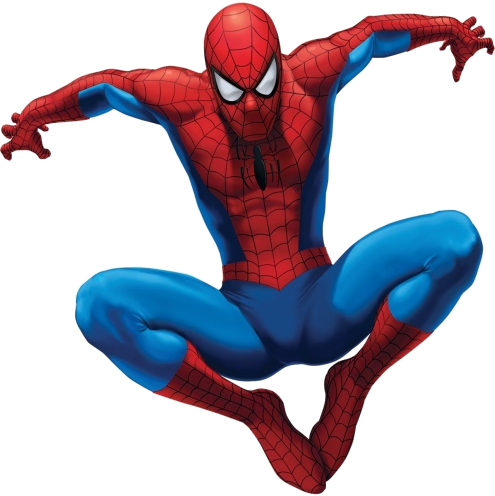
\includegraphics[height=2.9cm]{img/les2-hero-1}};
    \node[anchor=north] (hero2) at (0.8,2.05)
    {
\includegraphics[height=4cm]{img/les2-hero-2}};
    \node[anchor=north] (hero3) at (1.3,1.575)
    {
\includegraphics[height=3.1cm]{img/les2-hero-3}};
    \node[anchor=north] (hero4) at (1.8,2.1)
    {
\includegraphics[height=4.1cm]{img/les2-hero-4}};
    \node[anchor=north] (hero5) at (2.3,1.95)
    {
\includegraphics[height=3.8cm]{img/les2-hero-5}};

    \node (size1) at (0.3, 1.5) {\scriptsize 141 cm};
    \node (size2) at (0.8, 2.1) {\scriptsize 198 cm};
    \node (size3) at (1.3, 1.51) {\scriptsize 143 cm};
    \node (size4) at (1.8, 2.15) {\scriptsize 201 cm};
    \node (size5) at (2.3, 1.95) {\scriptsize 184 cm};
  \end{tikzpicture}
\end{frame}

\begin{frame}
  \frametitle{Sample and population}

  \begin{figure}
    \centering
    
\includegraphics[width=1.00\textwidth]{img/les5-heroes.jpg}
    \label{fig:les5-heroes}
  \end{figure}

\end{frame}

\begin{frame}
  \frametitle{Sample and population}
  \brightbox{ \textcolor{HoGentAccent6}{Population}: the set of all objects that we are interested in for our research}

  \brightbox{ \textcolor{HoGentAccent6}{Sample}: a subset from the population that is being researched more closely}

  \begin{center}
    \begin{tikzpicture}
      \fill[HoGentAccent4] (2,2) ellipse (4cm and 2 cm) ;
      \fill[HoGentAccent2] (2,2) ellipse (2cm and 1cm) ;
      \node[draw=none,minimum size=1cm,inner sep=0pt] at (3,0.5) {population};
      \node[draw=none,minimum size=1cm,inner sep=0pt] at (3,2) {sample};
    \end{tikzpicture}
  \end{center}
\end{frame}

\begin{frame}
  \frametitle{Sampling methods}
  \begin{center}
    \begin{tikzpicture}[
        auto, thick, ->, >=stealth', shorten >=1pt, node distance=2cm,
        fase/.style={ shape=rectangle, fill=HoGentFBO, text=white, draw}
      ]

    \node[fase] (1) { Definition of the population};
    \node[fase] (2) [below of=1] { Specifying a sampling frame };
    \node[fase] (3) [below of=2] { Time/budget considerations };

    \draw (1) -- (2);
    \draw (2) -- (3);
    \end{tikzpicture}
  \end{center}

\end{frame}

\begin{frame}
\frametitle{Stratified sampling}

\begin{center}
    \begin{tabular}{l|cccc|c}
        & \multicolumn{4}{c|}{\textbf{Age}} & \\
        Gender & $\le 18$ & $]18,25]$ & $]25, 40]$ & $> 40$ & Total\\
        \hline
        Female & 500 & 1500 & 1000 & 250 & 3250 \\
        Male   & 400 & 1200 & 800 & 160 & 2560\\
        \hline
        Total  & 900 & 2700 & 1800 & 410 & 5810
    \end{tabular}
    
    \vspace{1cm}
    
    \pause
    \begin{tabular}{l|cccc|c}
        & \multicolumn{4}{c|}{\textbf{Age}} & \\
        Gender & $\le 18$ & $]18,25]$ & $]25, 40]$ & $> 40$ & Total\\
        \hline
        Female & 50 & 150 & 100 & 25 & 325 \\
        Male   & 40 & 120 & 80 & 16 & 256\\
        \hline
        Total & 90 & 270 & 180 & 41 & 581
    \end{tabular}
    
\end{center}
\end{frame}

\begin{frame}
  \frametitle{Sampling methods}

  \begin{description}
    \item[Probability (or random) sampling]: each element from the population has an equal probability of being selected into the sample
    \item[Non-probability sampling]: 
    samples are \textit{not} randomly selected. Objects that can be easily collected are more likely to be included in the sample. (convenience sampling)
  \end{description}

  \begin{center}
    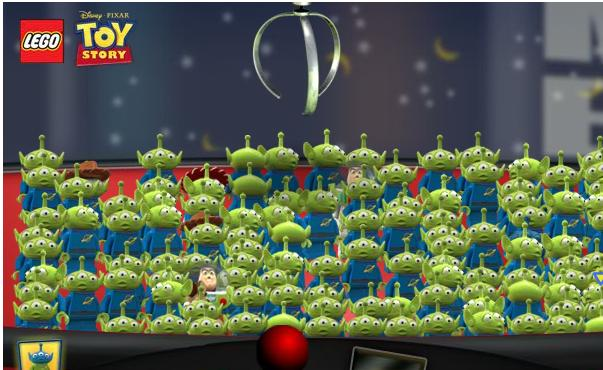
\includegraphics[width=.5\textwidth]{img/les4-aselect}
  \end{center}
\end{frame}

\begin{frame}
  \frametitle{Sample errors}

  \begin{itemize}
    \item<+-> Random sampling errors
      \begin{itemize}
        \item Random variations in the sampling due to random selection
      \end{itemize}
    \item<+-> Systematic sampling errors / Selection bias
      \begin{itemize}
        \item Online survey will not reach people without internet access
        \item Street survey is limited to the people that accidentally pass by
        \item Voluntary survey will select only people interested in the subject
      \end{itemize}
    \item<+-> Random non-sampling errors
      \begin{itemize}
        \item E.g.~respondent checked the wrong answer by mistake
      \end{itemize}
    \item<+-> Systematic non-sampling errors
      \begin{itemize}
\item Poor or non-calibrated measuring equipment (eg. poor balance)
\item Value can be influenced by the fact that you are measuring
\item Respondents may lie (number of cigarettes per day)
      \end{itemize}
  \end{itemize}
\end{frame}

\begin{frame}
  \frametitle{Variance and standard deviation of a sample}

  \begin{center}
    Adapted formula:

    \begin{equation*}
    s^2 = \frac{1}{\alert{n-1}} \sum_{i=1}^{n} (\overline{x} - x_i)^2
    \end{equation*}

    It is possible to prove mathematically why this is better,\\
    but we will study this empirically.

% applet no longer works
%    \vfill
%    Java applet: \url{http://www.uvm.edu/~dhowell/SeeingStatisticsApplets/N-1.html}

    \vfill
    R-script: \href{https://github.com/HoGentTIN/research-techniques-course/blob/master/syllabus/data/sample-variance.R}{syllabus/data/sample-variance.R}
  \end{center}
\end{frame}

\begin{frame}
\frametitle{Overview symbols}

{\tabulinesep=1.2mm
    \begin{tabu}{|r|c|c|}
        \hline
        & population & sample \\
        \hline
        number of objects & $N$ & $n$ \\
        \hline
        mean/average & $\mu$ & $\overline{x}$ \\
        \hline
        variance & $\sigma^2 = \frac{\sum (\mu-x_i)^2}{N}$ & $s^2  = \frac{\sum (\overline{x}-x_i)^2}{n-1}$ \\
        \hline
        standaarddeviation & $\sigma$ & $s$ \\
        \hline
\end{tabu}}
\end{frame}

\section{Probability distribution of a sample}

\begin{frame}
  \frametitle{Recap from probability theory}

  \begin{itemize}
    \item Sample space
    \item Outcome
    \item Event
    \item Probability space
  \end{itemize}

  \vfill

  \hfill 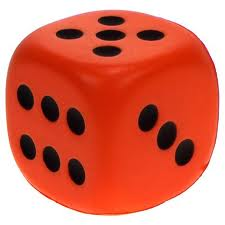
\includegraphics[width=.2\textwidth]{img/les04-dobbelsteen}
\end{frame}

%
\begin{frame}
  \frametitle{Probability distribution for a single die}
  
  What is the probability to throw a specific number with a single die?
  
  \begin{center}
    \begin{tabular}{|c|c|c|c|c|c|}
      \hline
      1&2&3&4&5&6\\
      \hline
      \onslide<2->{$\frac{1}{6}}$ &\onslide<2->{$\frac{1}{6}}$ &\onslide<2->{$\frac{1}{6}}$ &\onslide<2->{$\frac{1}{6}}$ &\onslide<2->{$\frac{1}{6}}$ &     \onslide<2->{$\frac{1}{6}}$ \\
      \hline
      
    \end{tabular}
  \end{center}
  \onslide<2->{%
  \begin{center}
  \begin{tikzpicture}
  \begin{axis}[ybar,ytick=data, anchor=north, bar width=1, yscale=.5]
  \addplot[fill=HoGentBlue]
  coordinates {
    (1, 1/6)
    (2, 1/6)
    (3, 1/6)
    (4, 1/6)
    (5, 1/6)
    (6, 1/6)};
  \end{axis}
  \end{tikzpicture}
\end{center}
}
\end{frame}

\begin{frame}
  \frametitle{Probability distribution for two dice}

  \begin{center}
    \begin{tabular}{|c|c|c|c|c|c|c|c|c|c|c|}
    	\hline
    	             2               &              3               &              4               &              5               &              6               &              7               &              8               &              9               &              10              &              11              &              12              \\ \hline
    	\onslide<2->{$\frac{1}{36}}$ & \onslide<2->{$\frac{2}{36}}$ & \onslide<2->{$\frac{3}{36}}$ & \onslide<2->{$\frac{4}{36}}$ & \onslide<2->{$\frac{5}{36}}$ & \onslide<2->{$\frac{6}{36}}$ & \onslide<2->{$\frac{5}{36}}$ & \onslide<2->{$\frac{4}{36}}$ & \onslide<2->{$\frac{3}{36}}$ & \onslide<2->{$\frac{2}{36}}$ & \onslide<2->{$\frac{1}{36}}$ \\ \hline
    \end{tabular}
  \end{center}

  \onslide<2->{%
    \begin{tikzpicture}
  \begin{axis}[ybar,ytick=data, anchor=north, bar width=1, yscale=.5]
  \addplot[fill=HoGentBlue]
  coordinates {
    (2, 1/36)
    (3, 2/36)
    (4, 3/36)
    (5, 4/36)
    (6, 5/36)
    (7, 6/36)
    (8, 5/36)
    (9, 4/36)
    (10, 3/36)
    (11, 2/36)
    (12, 1/36)
  };
  
  \end{axis}
  \end{tikzpicture}}

\end{frame}

  \pgfmathdeclarefunction{gauss}{2}{%
    \pgfmathparse{1/(#2*sqrt(2*pi))*exp(-((x-#1)^2)/(2*#2^2))}%
  }

\begin{frame}
  \frametitle{Continuous probability distribution}

  The probability distribution of Superman's reaction time $x$ in milliseconds:

  \vspace{1cm}

  \begin{tikzpicture}
\begin{axis}[
  domain=0:10, samples=100,
  axis lines*=left, xlabel=$x$ (ms), ylabel=$y$,
  every axis y label/.style={at=(current axis.above origin),anchor=south},
  every axis x label/.style={at=(current axis.right of origin),anchor=west},
  height=5cm, width=11cm,
  xtick={5,3.5,6.5}, ytick=\empty,
  enlargelimits=false, clip=false, axis on top,
  grid = major
  ]
  \addplot [fill=cyan!20, draw=none, domain=0:9] {gauss(5,1.5)} \closedcycle;
  \draw [yshift=-0.6cm, latex-latex](axis cs:3.5,0) -- node [fill=white] {$\sigma$} (axis cs:4.99,0);
  \draw [yshift=-0.6cm, latex-latex](axis cs:5.01,0) -- node [fill=white] {$\sigma$} (axis cs:6.5,0);
  \draw [-](axis cs:5,-0.035) -- (axis cs:5,-0.06);
  \node at (axis cs:5,-0.075) {$\mu$};
  \end{axis}
  \end{tikzpicture}
  \hfill
\includegraphics[width=1.5cm]{img/les2-hero-3}
\end{frame}

\begin{frame}
\frametitle{\textit{Standard} normal distribution and the $z$-score}
\centering
\begin{columns}[c]
    \column{.5\textwidth}
Normal distribution\\
$x \in X \sim Nor(\mu, \sigma)$\\
    \begin{tikzpicture}
    \begin{axis}[
    domain=-2.5:2.5,
    axis lines*=left,
    xmin=-2.5, xmax=2.5,
    ymin=0, ymax=0.39,
    xlabel=$X$,
    every axis x label/.style={at=(current axis.right of origin),anchor=west},
    every axis y label/.style={at=(current axis.above origin),anchor=south},
    height=4cm, width=6cm,
    xtick={-1.4,0,1.4},
    xticklabels={$\mu-\sigma$,$\mu$,$\mu+\sigma$},
    ytick=\empty,
    enlargelimits=false,
    axis on top,
    clip=false,
    ]
    \addplot[very thick,smooth,draw=HoGentFBO]{gauss(0,1.4)};
    \draw [-](axis cs:0.4,0) -- (axis cs:0.4,0.274); %vertical line
    \node at (axis cs: 0.56,0.1) {$x$}; %label x
    \draw [latex-latex](axis cs:2.2,0.22) -- (axis cs:3.5,0.22);
    \end{axis}
    \end{tikzpicture}
    \column{.5\textwidth}
\textbf{\textit{Standard}} normal distribution\\
$z \in Z \sim Nor(0, 1)$\\
    \begin{tikzpicture}
    \begin{axis}[
    domain=-2.5:2.5,
    axis lines*=left,
    xmin=-2.5, xmax=2.5,
    ymin=0, ymax=0.39,
    xlabel=$Z$,
    every axis x label/.style={at=(current axis.right of origin),anchor=west},
    every axis y label/.style={at=(current axis.above origin),anchor=south},
    height=4cm, width=6cm,
    xtick={-1,0,1},
    enlargelimits=false,
    axis on top,
    clip=false,
    ]
    \addplot[very thick,smooth,draw=HoGentFBO]{gauss(0,1)};
    \draw [-](axis cs:0.286,0) -- (axis cs:0.286,0.383); %vertical line
    \node at (axis cs: 0.42,0.12 ) {$z$}; %label z
    \end{axis}
    \end{tikzpicture}
\end{columns}

\vfill
$x$ and $z$ have an equivalent position on the Gauss-curve.\\
What is the mathematical relation between $x$ and $z$?
\vfill
\pause
{\Large $x = \mu + z . \sigma$} ~~~ and ~~~ {\Large $z = \frac{x - \mu}{\sigma}$}
\end{frame}

\begin{frame}
  \frametitle{Standard normal distribution}

  % Source: http://johncanning.net/wp/?p=1202
  \begin{center}
    \begin{tikzpicture}
      \begin{axis}[
          no markers, domain=0:10, samples=100,
          axis lines*=left,height=6cm, width=10cm,
          xtick={-3, -2, -1, 0, 1, 2, 3}, ytick=\empty,
          enlargelimits=false, clip=false, axis on top,
          grid = major
        ]
        \addplot [smooth,fill=cyan!20, draw=none, domain=-3:3] {gauss(0,1)} \closedcycle;
        \addplot [smooth,fill=orange!20, draw=none, domain=-3:-2] {gauss(0,1)} \closedcycle;
        \addplot [smooth,fill=orange!20, draw=none, domain=2:3] {gauss(0,1)} \closedcycle;
        \addplot [smooth,fill=blue!20, draw=none, domain=-2:-1] {gauss(0,1)} \closedcycle;
        \addplot [smooth,fill=blue!20, draw=none, domain=1:2] {gauss(0,1)} \closedcycle;
        \addplot[<->] coordinates {(-1,0.4) (1,0.4)};
        \addplot[<->] coordinates {(-2,0.3) (2,0.3)};
        \addplot[<->] coordinates {(-3,0.2) (3,0.2)};
        \node[coordinate, pin={68.3\%}] at (axis cs: 0, 0.35){};
        \node[coordinate, pin={95.4\%}] at (axis cs: 0, 0.25){};
        \node[coordinate, pin={99.7\%}] at (axis cs: 0, 0.15){};
        \node[coordinate, pin={34.1\%}] at (axis cs: -0.5, 0){};
        \node[coordinate, pin={34.1\%}] at (axis cs: 0.5, 0){};
        \node[coordinate, pin={13.6\%}] at (axis cs: 1.5, 0){};
        \node[coordinate, pin={13.6\%}] at (axis cs: -1.5, 0){};
        \node[coordinate, pin={2.1\%}] at (axis cs: 2.5, 0){};
        \node[coordinate, pin={2.1\%}] at (axis cs: -2.5, 0){};
      \end{axis}
    \end{tikzpicture}
  \end{center}
\end{frame}

\begin{frame}[fragile]
\frametitle{Most important R functions}

A normal distribution with mean \texttt{m} and standard deviation \texttt{s}:
\vfill
\centering
\begin{tabular}{ll}
    \textbf{Function}     & \textbf{Return value}                       \\ \hline
    \verb|pnorm(x, m, s)| & Left tail probability, $P(X<\mathtt{x})$         \\
    \verb|dnorm(x, m, s)| & Height of the Gauss curve at \texttt{x} \\
    \verb|qnorm(p, m, s)| & Under what limit will \texttt{p}\% of the   \\
    & observations be situated?                        \\
    \verb|rnorm(n, m, s)| & Generate \texttt{n} normally distributed randon numbers
\end{tabular}
\vfill
\texttt{pnorm(x) = pnorm(x,0,1)} : \textit{\textbf{standard}} normal distribution is the default
\end{frame}

\begin{frame}
\frametitle{Calculating probabilities}
What is the probability that \dots\\
\ldots Superman's response time is more than 6 milliseconds?
\vfill
Math. notation:\\
\hspace{1cm}$P( X > 6)$ = ?\hspace{1cm}with $X \sim Nor(\mu=5,\sigma=1,5)$
\vfill
\begin{tikzpicture}
\begin{axis}[
domain=0:10,
axis lines*=left,
xlabel=$x$,
every axis x label/.style={at=(current axis.right of origin),anchor=west},
every axis y label/.style={at=(current axis.above origin),anchor=south},
height=5cm, width=8cm,
xtick={3.5,5,6.5},
ytick=\empty,
enlargelimits=false,
axis on top,
clip=false,
]
\addplot[fill=cyan!20, draw=black, domain=6:10] {gauss(5,1.5)} \closedcycle;
\addplot[very thick,smooth,draw=HoGentFBO]{gauss(5,1.5)};
\draw [-latex](axis cs:7,0.05) -- (axis cs:8.5,0.1);
\node at (axis cs: 10, 0.1) {$P(X>6)$};
\draw [-](axis cs:6,-0.005) -- (axis cs:6,-0.040);
\node at (axis cs: 6, -0.055) {$6$};
\end{axis}
\end{tikzpicture}
\end{frame}

\begin{frame}
  \frametitle{Calculating probabilities}
  $P( X > 6)$ = ?\hspace{1cm}with $X \sim Nor(\mu=5,\sigma=1,5)$
  \vfill
  \begin{enumerate}
  \item Old school, with $z$-score
    \begin{itemize}
      \pause
      \item convert to $z$-score\\
      $z=\frac{6-5}{1.5}=0.667$ so $P(X>6) = P(Z>0.667)$
      \item convert to a \textbf{\textit{left}} tail probability
      \begin{itemize}
          \item 100\% probability rule: $P(Z>0.667)=1-P(Z<0.667)$
          \item or symmetry rule: $P(Z>0.667)=P(Z<-0.667)$
      \end{itemize}
      \item look up in a $z$-table
      (eg. \url{http://sixsigmastudyguide.com/wp-content/uploads/2014/04/z-table.jpg})
      or calculate in R (\texttt{1-pnorm(0.667)})
  \end{itemize}
  \vfill
  \item Direct calculation with R (or calculator)
  \begin{itemize}
      \pause
      \item first convert to a \textbf{\textit{left}} tail probability:\\
      with the 100\% probability rule: $P(X>6)=1-P(X<6)$
      \item calculate with R: $1-P(X<6)=$\texttt{1-pnorm(6,5,1.5)}
  \end{itemize}
  \end{enumerate}
\end{frame}

\begin{frame}
  \frametitle{Application}

  What is the probability that Superman's reaction time is

  \begin{enumerate}
    \item Less than 4 ms?
    \item More than 7 ms?
    \item Less than 3 ms?
    \item Between 2 and 6.5 ms?
    \item Under what time limit is 80\% of his reaction times?
  \end{enumerate}
\end{frame}

\begin{frame}
  \frametitle{Question 3: $P(X<3)$}

  \begin{tikzpicture}
  \begin{axis}[no markers,domain=-4:4,axis lines*=left,yscale=.7,enlargelimits=false,clip=false]
    \addplot[very thick,smooth,draw=HoGentFBO]{gauss(0, 1)};
    \addplot[smooth,fill=black!20, draw=black, domain=-4:-4/3] {gauss(0,1)} \closedcycle;

    \node at (axis cs: -1.33, -.05) {\small -1.33};
  \end{axis}
  \end{tikzpicture}
\end{frame}

\begin{frame}
  \frametitle{Question 4: $P(2<X<6,5)$}

  \begin{tikzpicture}
  \begin{axis}[no markers,domain=-4:4,axis lines*=left,yscale=.7,enlargelimits=false,clip=false]
    \addplot[very thick,smooth,draw=HoGentFBO]{gauss(0, 1)};
    \addplot[smooth,fill=black!20, draw=black, domain=-2:1] {gauss(0,1)} \closedcycle;

    \node at (axis cs: 1, -.05) {\small 1};
  \end{axis}
  \end{tikzpicture}
\end{frame}

\begin{frame}
  \frametitle{Question 5}

  For what value of $x$ is $P(X<x) = 80\%$?

  \vfill

  \begin{tikzpicture}
  \begin{axis}[no markers,domain=-4:4,axis lines*=left,yscale=.7,enlargelimits=false,clip=false]
    \addplot[very thick,smooth,draw=HoGentFBO]{gauss(0, 1)};
    \addplot[smooth,fill=black!20, draw=black, domain=-4:.84] {gauss(0,1)} \closedcycle;

    \node at (axis cs: .84, -.05) {\small .84};
  \end{axis}
  \end{tikzpicture}
\end{frame}

\section{The central limit theorem}
\sectionframelogo{}

\begin{frame}
  \frametitle{The central limit theorem}

  \brightbox{If the sample size is sufficiently large, then the probability distribution of the arithmetic mean will be approximately normally distributed, regardless of the underlying distribution of the population.}

  \vfill

  \begin{columns}[c]
    \column{.33\textwidth}
    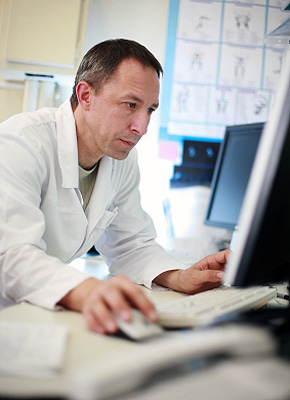
\includegraphics[width=2cm]{img/les4-centrlimiet}
    \column{.33\textwidth}
    \begin{itemize}
      \item 1 test
      \item 25 tests
      \item 100 tests
    \end{itemize}
    \column{.33\textwidth}
    
\includegraphics[width=2cm]{img/les2-hero-3}
  \end{columns}

\vfill
Demo: \url{https://students.brown.edu/seeing-theory/probability-distributions/index.html}

\end{frame}

\begin{frame}
  \frametitle{The central limit theorem}

  Consider a random sample of $n$ observations from an arbitrary distributed population with expected value $\mu$ and standard deviation $\sigma$. If $n$ is sufficiently large, the probability of $\overline{x}$ will approximate a normal distribution with mean $\mu_{\overline{x}} = \mu$ and standard deviation $\sigma_{\overline{x}} = \frac{\sigma}{\sqrt{n}}$.

\vspace{0.4cm}
  The larger the sample, the better the distribution of $\overline{x}$ will match a normal distribution.
\end{frame}

\section{From sample to population}
\sectionframelogo{}

\begin{frame}
  \frametitle{Point estimate}
  \brightbox{A \textcolor{HoGentYellow}{point estimate} for a population parameter is an estimate for that parameter based on a sample (subset) of the population.}
\vfill
  \textbf{Example}: $\overline{x}$ is a \textbf{point estimate} for $\mu$
\vfill
  $\overline{x}$ is the mean of a sample\\
  $\mu$ is the mean of the entire population
\end{frame}

\subsection{Confidence intervals}

\begin{frame}
  \frametitle{Confidence interval}
  \brightbox{A \textcolor{HoGentYellow}{confidence interval} for a population parameter is an interval that will contain the value of that parameter with a specific \textcolor{HoGentYellow}{confidence level}. }
\vfill
\textbf{Example}: $\mu \in [a,b]$ with a confidence level of 95\%
\vfill
  $\mu$ is the mean of the entire population\\
  $[a,b]$ is the confidence interval
\end{frame}

\subsection{Confidence interval for large samples}

\begin{frame}
  \frametitle{Confidence interval for large samples}
Given a sample with mean $\overline{x}$.\\
We are looking for an interval $\left[ ~\overline{x}-b~,~\overline{x}+b~\right]$ for which we can say with a confidence level $(1-\alpha)$ of for example 95\% that $\mu$ is inside this interval.
\vfill
\[ P\left( \overline{x}-b < \mu < \overline{x}+b \right) = 1-\alpha = 0,95 \]
\vfill
\begin{tikzpicture}
\begin{axis}[
domain=-3:3,
axis lines*=left,
height=5cm, width=12cm,
xtick={-1.96,0,1.96},
xticklabels={$\overline{x}-b$,$\overline{x}$,$\overline{x}+b$},
ytick=\empty,
enlargelimits=false,
axis on top,
clip=false,
]
\addplot[fill=cyan!20, draw=black, domain=-1.96:1.96] {gauss(0,1)} \closedcycle;
\addplot[very thick,smooth,draw=HoGentFBO]{gauss(0,1)};
%\addplot[smooth,dashed,draw=HoGentFBO]{gauss(0.8,1)};
\node [text width=1.5cm,fill=cyan!20,align=center] at (axis cs: 0, 0.17) {95\%\\($1-\alpha$)};
\draw [-latex](axis cs:2.15,0.02) -- (axis cs:2.4,0.07);
\node [text width=1cm,fill=white,align=center] at (axis cs: 2.5,0.14) {2,5\%\\($\frac{\alpha}{2}$)};
\draw [-latex](axis cs:-2.15,0.02) -- (axis cs:-2.3,0.07);
\node [text width=1cm,align=center] at (axis cs: -2.3,0.14) {2,5\%\\($\frac{\alpha}{2}$)};
\draw [-](axis cs:0.6,0.02) -- (axis cs:0.6,-0.06);
\node [align=center] at (axis cs: 0.6,-0.09) {$\mu$};
\end{axis}
\end{tikzpicture}
\end{frame}

\begin{frame}
\frametitle{Confidence interval for large samples}
Because of the central limit theorem we know:
\[ \overline{x} \in \overline{X} \sim Nor(\mu,\frac{\sigma}{\sqrt{n}}) \]

\vfill
And because of the symmetry we can say:
\[ P\left( \overline{x}-b < \mu < \overline{x}+b \right) = P\left( \mu-b < \overline{x} < \mu+b \right) \]

\vfill
\begin{tikzpicture}

\begin{axis}[
domain=-3:3,
axis lines*=left,
height=5cm, width=12cm,
xlabel=$\overline{X}$,
every axis x label/.style={at=(current axis.right of origin),anchor=west},
every axis y label/.style={at=(current axis.above origin),anchor=south},
xtick={-1.36,-0.4,0.6,1.6,2.56},
xticklabels={$\mu-b$,,$\mu$,,$\mu+b$},
ytick=\empty,
enlargelimits=false,
axis on top,
clip=false,
]
\addplot[fill=cyan!20, draw=black, domain=-1.36:2.56] {gauss(0.6,1)} \closedcycle;
\addplot[very thick,smooth,draw=HoGentFBO]{gauss(0.6,1)};
\addplot[smooth,dashed,draw=HoGentFBO]{gauss(0,1)};
\node [text width=1.5cm,align=center] at (axis cs: 0.6, 0.17) {95\%\\($1-\alpha$)};
\draw [-latex](axis cs:2.75,0.02) -- (axis cs:3.0,0.07);
\node [text width=1cm,fill=white,align=center] at (axis cs: 3.1,0.14) {2,5\%\\($\frac{\alpha}{2}$)};
\draw [-latex](axis cs:-1.55,0.02) -- (axis cs:-1.7,0.07);
\node [text width=0.8cm,fill=white,align=center] at (axis cs: -1.8,0.14) {2,5\%\\($\frac{\alpha}{2}$)};
\draw [-,dashed](axis cs:0,0.4) -- (axis cs:0,-0.07);
\node [align=center] at (axis cs: 0,-0.1) {$\overline{x}$};
\draw [latex-latex](axis cs:0.6,-0.07) -- node [fill=white] {$\frac{\sigma}{\sqrt{n}}$} (axis cs:1.6,-0.07);
\end{axis}
\end{tikzpicture}

\end{frame}

\begin{frame}
\frametitle{Confidence interval for large samples}

We will now calculate the $z$-score for $\overline{x}$:
\[ z = \frac{\overline{x} - \mu}{\frac{\sigma}{\sqrt{n}}} \]

\vfill
We lookup (or calculate) the value $z_\frac{\alpha}{2}$ for which:
\[ P\left(-z_{\frac{\alpha}{2}} < z < z_{\frac{\alpha}{2}}\right) = 1 - \alpha = 0.95 \]
\[ P\left(z < z_{\frac{\alpha}{2}}\right) = 1 - \frac{\alpha}{2} = 0.975 \]
\[ z_{\frac{\alpha}{2}} = \texttt{qnorm(0.975)} \approx 1.96 \]

\vfill
\begin{tikzpicture}
\begin{axis}[
domain=-3:3,
axis lines*=left,
xlabel=$Z$,
every axis x label/.style={at=(current axis.right of origin),anchor=west},
every axis y label/.style={at=(current axis.above origin),anchor=south},
height=4cm, width=10cm,
xtick={-1.96,-1,0,1,1.96},
xticklabels={-$z_\frac{\alpha}{2}$,-1,0,1,$z_\frac{\alpha}{2}$},
ytick=\empty,
enlargelimits=false,
axis on top,
clip=false,
]
\addplot[fill=cyan!20, draw=black, domain=-1.96:1.96] {gauss(0,1)} \closedcycle;
\addplot[very thick,smooth,draw=HoGentFBO]{gauss(0,1)};
\node [text width=1.5cm,align=center] at (axis cs: 0, 0.15) {95\%\\($1-\alpha$)};
\draw [-latex](axis cs:2.15,0.02) -- (axis cs:2.4,0.07);
\node [text width=1cm,align=center] at (axis cs: 2.5,0.16) {2,5\%\\($\frac{\alpha}{2}$)};
\draw [-latex](axis cs:-2.15,0.02) -- (axis cs:-2.3,0.07);
\node [text width=1cm,align=center] at (axis cs: -2.3,0.16) {2,5\%\\($\frac{\alpha}{2}$)};

\end{axis}
\end{tikzpicture}

\end{frame}

\begin{frame}
\frametitle{Confidence interval for large samples}

We now get:
\[ P\left(-1.96 < \frac{\overline{x} - \mu}{\frac{\sigma}{\sqrt{n}}} < 1.96 \right) = 0.95 \]
\[ P\left( \mu-1.96 \cdot \frac{\sigma}{\sqrt{n}} < \overline{x} < \mu+1.96 \cdot \frac{\sigma}{\sqrt{n}} \right)  = 0.95 \]

Because of symmetry we can swap $\mu$ and $\overline{x}$:
\[ P\left( \overline{x}-1.96 \cdot \frac{\sigma}{\sqrt{n}} < \mu < \overline{x}+1.96 \cdot  \frac{\sigma}{\sqrt{n}} \right)  = 0.95 \]

Now we can say with 95\% confidence that:
\[ \mu \in \left[~\overline{x}-1.96 \cdot \frac{\sigma}{\sqrt{n}}~,~\overline{x}+1.96 \cdot  \frac{\sigma}{\sqrt{n}}~\right] \]

\small (in practice we will use $s_{sample}$ as an estimate for $\sigma_{population}$)

\end{frame}


\subsection{Confidence interval for small samples}

\begin{frame}
\frametitle{Student t-distribution for \textit{small} samples}
For a \textit{\textbf{small}} sample the central limit theorem is \textbf{no longer} valid.
\vfill
Instead we can say:\\
\vfill
If a population $X$ has a normal distribution $(X \sim Nor(\mu,\sigma))$\\
and you take a \textit{small} sample with mean $\overline{x}$ and standard deviation $s$, then
\[ t = \frac{\overline{x} - \mu}{\frac{s}{\sqrt{n}}} \]
will behave as a t-distribution with ~$n-1$~ degrees of freedom
\end{frame}

\begin{frame}
\frametitle{Student t-distribution for \textit{small} samples}
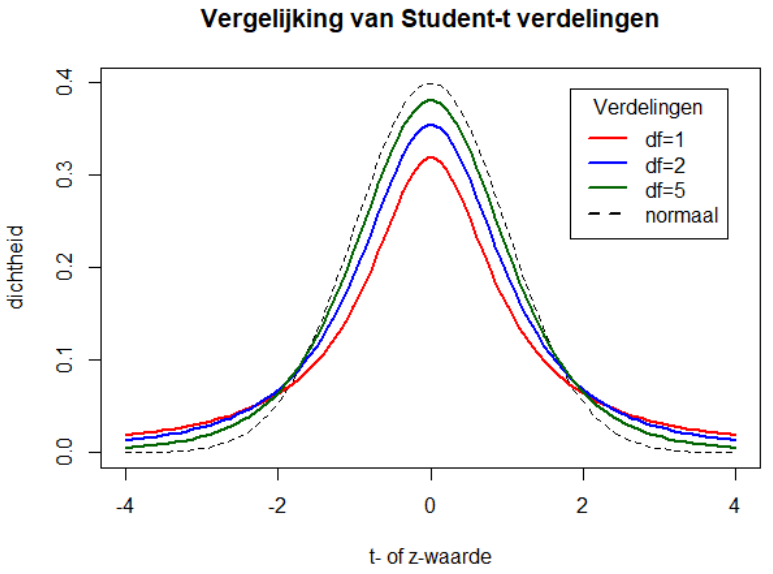
\includegraphics[width=\linewidth]{img/les04-t-distrib}
\end{frame}


\begin{frame}[fragile]
\frametitle{Student $t$-distribution in R}

For a $t$-distribution with ~\texttt{df}~ degrees of freedom:\\
\vfill
\centering
\begin{tabular}{ll}
    \textbf{Function} & \textbf{Return value}                                    \\ \hline
    \verb|pt(x, df)| & Left tail probability, $P(X<\mathtt{x})$                  \\
    \verb|dt(x, df)| & Height of the curve at \texttt{x}                     \\
    \verb|qt(p, df)| & Under what limit will \texttt{p}\% of the     \\
    & obsevations be situated?                             \\
    \verb|rt(n, df)| & Generate \texttt{n} random numbers with this distribution
\end{tabular}
\end{frame}

\begin{frame}
\frametitle{Confidence interval for \textit{small} samples}
To determine the confidence interval for the mean $\mu$ of a population, based on a \textit{small} sample, we first calculate $t_ {\frac{\alpha}{2},df}$.

\vfill
With a confidence level of 95\% we have $\frac{\alpha}{2}=0,025$\\
Assume for example $n=5$ (so \texttt{df=4}), then we have
\[ t_ {\frac{\alpha}{2},df} = \texttt{qt(0.975,4)} = 2.776 \]

\vfill
We can say with a certainty of 95\% that:
\[ \mu \in \left[~ \overline{x} - t_{\frac{\alpha}{2},df} \cdot \frac{s}{\sqrt{n}} ~,~ \overline{x} + t_{\frac{\alpha}{2},df} \cdot \frac{s}{\sqrt{n}} ~\right] \]

\end{frame}

\subsection{Confidence interval for a fraction}

\begin{frame}
  \frametitle{Confidence interval for a fraction}
  \[ \overline{p} = \frac{\textnormal{number of successes}}{n} \]
  \begin{itemize}
  \item The expected value of the probability distribution of $p$ is estimated by $\overline{p}$.
  \item The stdev of $p$ is estiamted by $\sqrt{\frac{\overline{p} \cdot (1-\overline{p})}{n}}$
  \item For large samples, $\overline{p}$ is approximately normally distributed
\end{itemize}

Since $\overline{p}$ is a sample mean of the number of successes, this allows us to draw a confidence interval analogous to the previously discussed interval estimate of $\mu$ for large samples.

  \[ p \in \left[~ \overline{p} - z_{\frac{\alpha}{2}} \cdot \sqrt{\frac{\overline{p} \cdot (1-\overline{p})}{n}} ~,~ \overline{p} + z_{\frac{\alpha}{2}} \cdot \sqrt{\frac{\overline{p} \cdot (1-\overline{p})}{n}} ~\right] \]
\end{frame}

\end{document}
